\section{Трансформеры}

Теперь, когда мы познакомились с механизмом внимания, напрашивается логичный вопрос: 
нужны ли нам вообще теперь LSTM? Как оказалось - нет. В своей фундаментальной работе 
"Attention Is All You Need" \cite{vaswani2017attention}, Vaswani et al. представили 
новую архитекутуру нейронной сети, \textbf{трансформер}, основанный исключительно на 
механизмах внимания, полностью отказываясь от рекуррентности и сверток. 

С момента своей первой публикации, трансформер обошел большинство моделей 
глубого обучение, прежде считавшиееся лучшими в своей сфере. Нынче архитекутура 
трансформера считается лидирующей во многих областях глубого обучения и потому 
представляет для нас особый интерес.

% Position Transformers as the modern “go-to” for long-horizon forecasting.

\subsection{Архитектура «с высока»}

Ключевая проблема рекуррентных нейронных сетей, LSTMs и GRU считавшихся передовыми 
подходами для моделирования последовательностей на момент выхода статьи \cite{vaswani2017attention} 
кроется в их последовательной природе. Обобщая, они генерируют последовательность скрытых 
состояний $h_t$, как функцию предыдщего скрытых состояний $h_{t-1}$ и входа для позиции 
$t$. Подобная последовательная природа исключает распараллеливание внутри обучающих 
примеров, что становится критичным при бОльших длинах последовательностей. Подобное 
ограничение и послужило вдохновением для трансформера - архитектуры модели, 
которая отказывается от рекуррентности и полностью полагается на механизм 
внимания для установления глобальных зависимостей между входом и выходом.

С высока, архитектура классического трансформера, представленного в 
"Attention Is All You Need" \cite{vaswani2017attention} представлена 
на рис. \ref{fig:the_transformer}. 

\begin{figure}[h!]
    \centering
    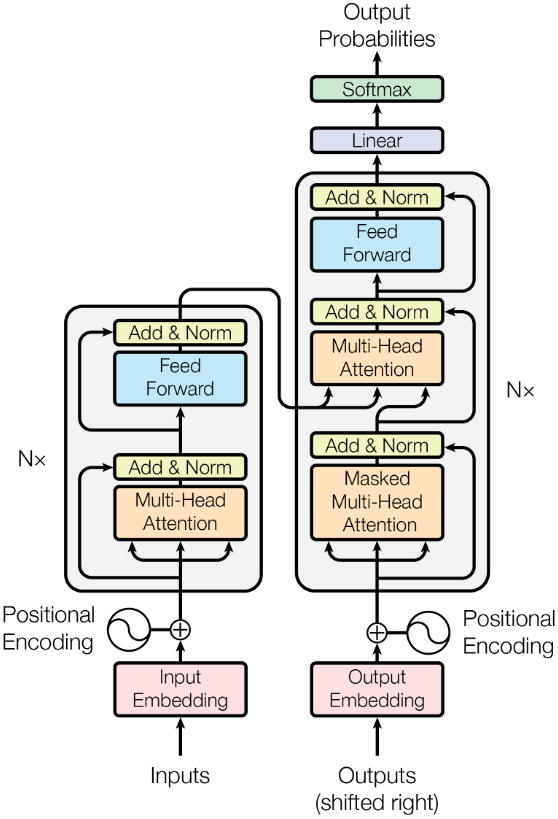
\includegraphics[width=0.6\textwidth, keepaspectratio]{the_transformer.png}
    \caption{Архитектура модели Трансформер. (Изначально, в своей статье 
    "Attention Is All You Need", модель трансформера была спроектирована для 
    задачи машинного перевода, из-за чего на диаграмме изображены слои эмбеддингов, 
    однако мы на них не будем акцентировать внимания. Нас сейчас больше интересует 
    архитекутра самой модели, ведь поняв ее, мы сможем легко обобщить 
    архитектуру трансформера для решения проблемы прогнозирования временных 
    рядов).}
    \label{fig:the_transformer}
\end{figure}

Представленная архитектура адаптирована для модели кодировщика-декодера 
(см. главу {\color{red} todo}), однако трансформер может состоять как только из 
левой части, т.е. кодировщика, так и правой, т.е. декодера, как мы это позже 
увидим в моделях BERT и GPT (см. главы {\color{red} todo} и {\color{red} todo}). 
Архитектура трансформера определяется общим механизмом, включающим в себя 
внимание и прямое распространение (attention-plus-feed-forward).

\subsection{Ключевые компоненты} % Core Building Blocks (Строительные блоки)

В отличии от ранее расмотренных LSTM, трансформер имеет гораздо более 
структурированную архитектуру и можно представить, что мы собираем его 
из нескольких строительных блоков.

\subsubsection{Внимание}

Функцию внимания можно описать как отображение \textbf{запроса (query)} 
и набора \textbf{пар ключ-значение (key-value pairs)} в \textbf{выход (output)}, 
где запрос, ключи, значения и выход - векторы. Выход находится как 
взвешенная сумма значений, где вес, присваивающийся каждому значению 
вычисляется функцией совместимости запроса с соответствующим ключом 
\cite{vaswani2017attention}. 

Одним известным подходом к вычислению совместимости (сходства) между двумя значениями 
является \textbf{косинусово сходство (cosine similarity)}:
\begin{equation*}
    \cos(\theta) = \cfrac{\bm{A} \cdot \bm{B}}{|| \bm{A} || || \bm{B} ||} = 
    \cfrac{\sum_{i=1}^n A_i B_i}{\sqrt{\sum_{i=1}^n A_i^2 \sqrt{\sum_{i=1}^n B_i^2}}}
\end{equation*}

Однако, чаще сходство в контексте механизма внимания рассчитывают несколько иначе - 
берут только числитель косинусова сходства, т.е. скалярное 
произведение $\bm{A} \cdot \bm{B}$. Т.к. знаменатель всего навсего 
нормирует значения, чтобы они были в диапазоне от -1 до 1, что в данном случае нам не 
особо нужно. 

В своей работе, Vaswani et al. рассчитывают внимание следующим образом:
\begin{equation*}
    \text{Attention($Q$, $K$, $V$)} = \text{softmax} \left( \cfrac{Q K^T}{\sqrt{d_k}} \right) V,
\end{equation*}
где $Q, K, V$ - матрицы запросов, ключей и значений соответственно (результат 
также представляет из себя матрицу).

Здесь, мы как раз и видим, что сходство между запросом и ключом находится из 
скалярного произведения (плюс масштабирующий коэффициент $\frac{1}{\sqrt{d_k}}$, 
который на практике помагает численной устойчивости). Затем применяется функция 
\text{sofmax} для получения весов для значений.

В контексте модели кодировщика-декодера, обычно механизм внимания разделяют на 
два: \textbf{self-attention} и \textbf{cross-attention}:
\begin{itemize}
    \item \textbf{self-attention}: значит, что мы рассчитываем сходство между элементами 
    \textit{внутри} последовательности (например при обработке последовательности 
    слов в предложении, self-attention как бы закодирует контекст, т.е. то, как 
    слова влияют друг на друга).
    \item \textbf{cross-attention}: значит, что мы рассчитываем сходство между 
    элементами \textit{между} последовательностями (например в задаче машинного перевода, 
    cross-attention закодирует сходство между словами в предложении на одном языке и 
    его переводе на другом языке).
\end{itemize}

\begin{figure}[h!]
    \centering
    \fbox{\begin{varwidth}{\dimexpr\textwidth-2\fboxsep-2\fboxrule\relax}
        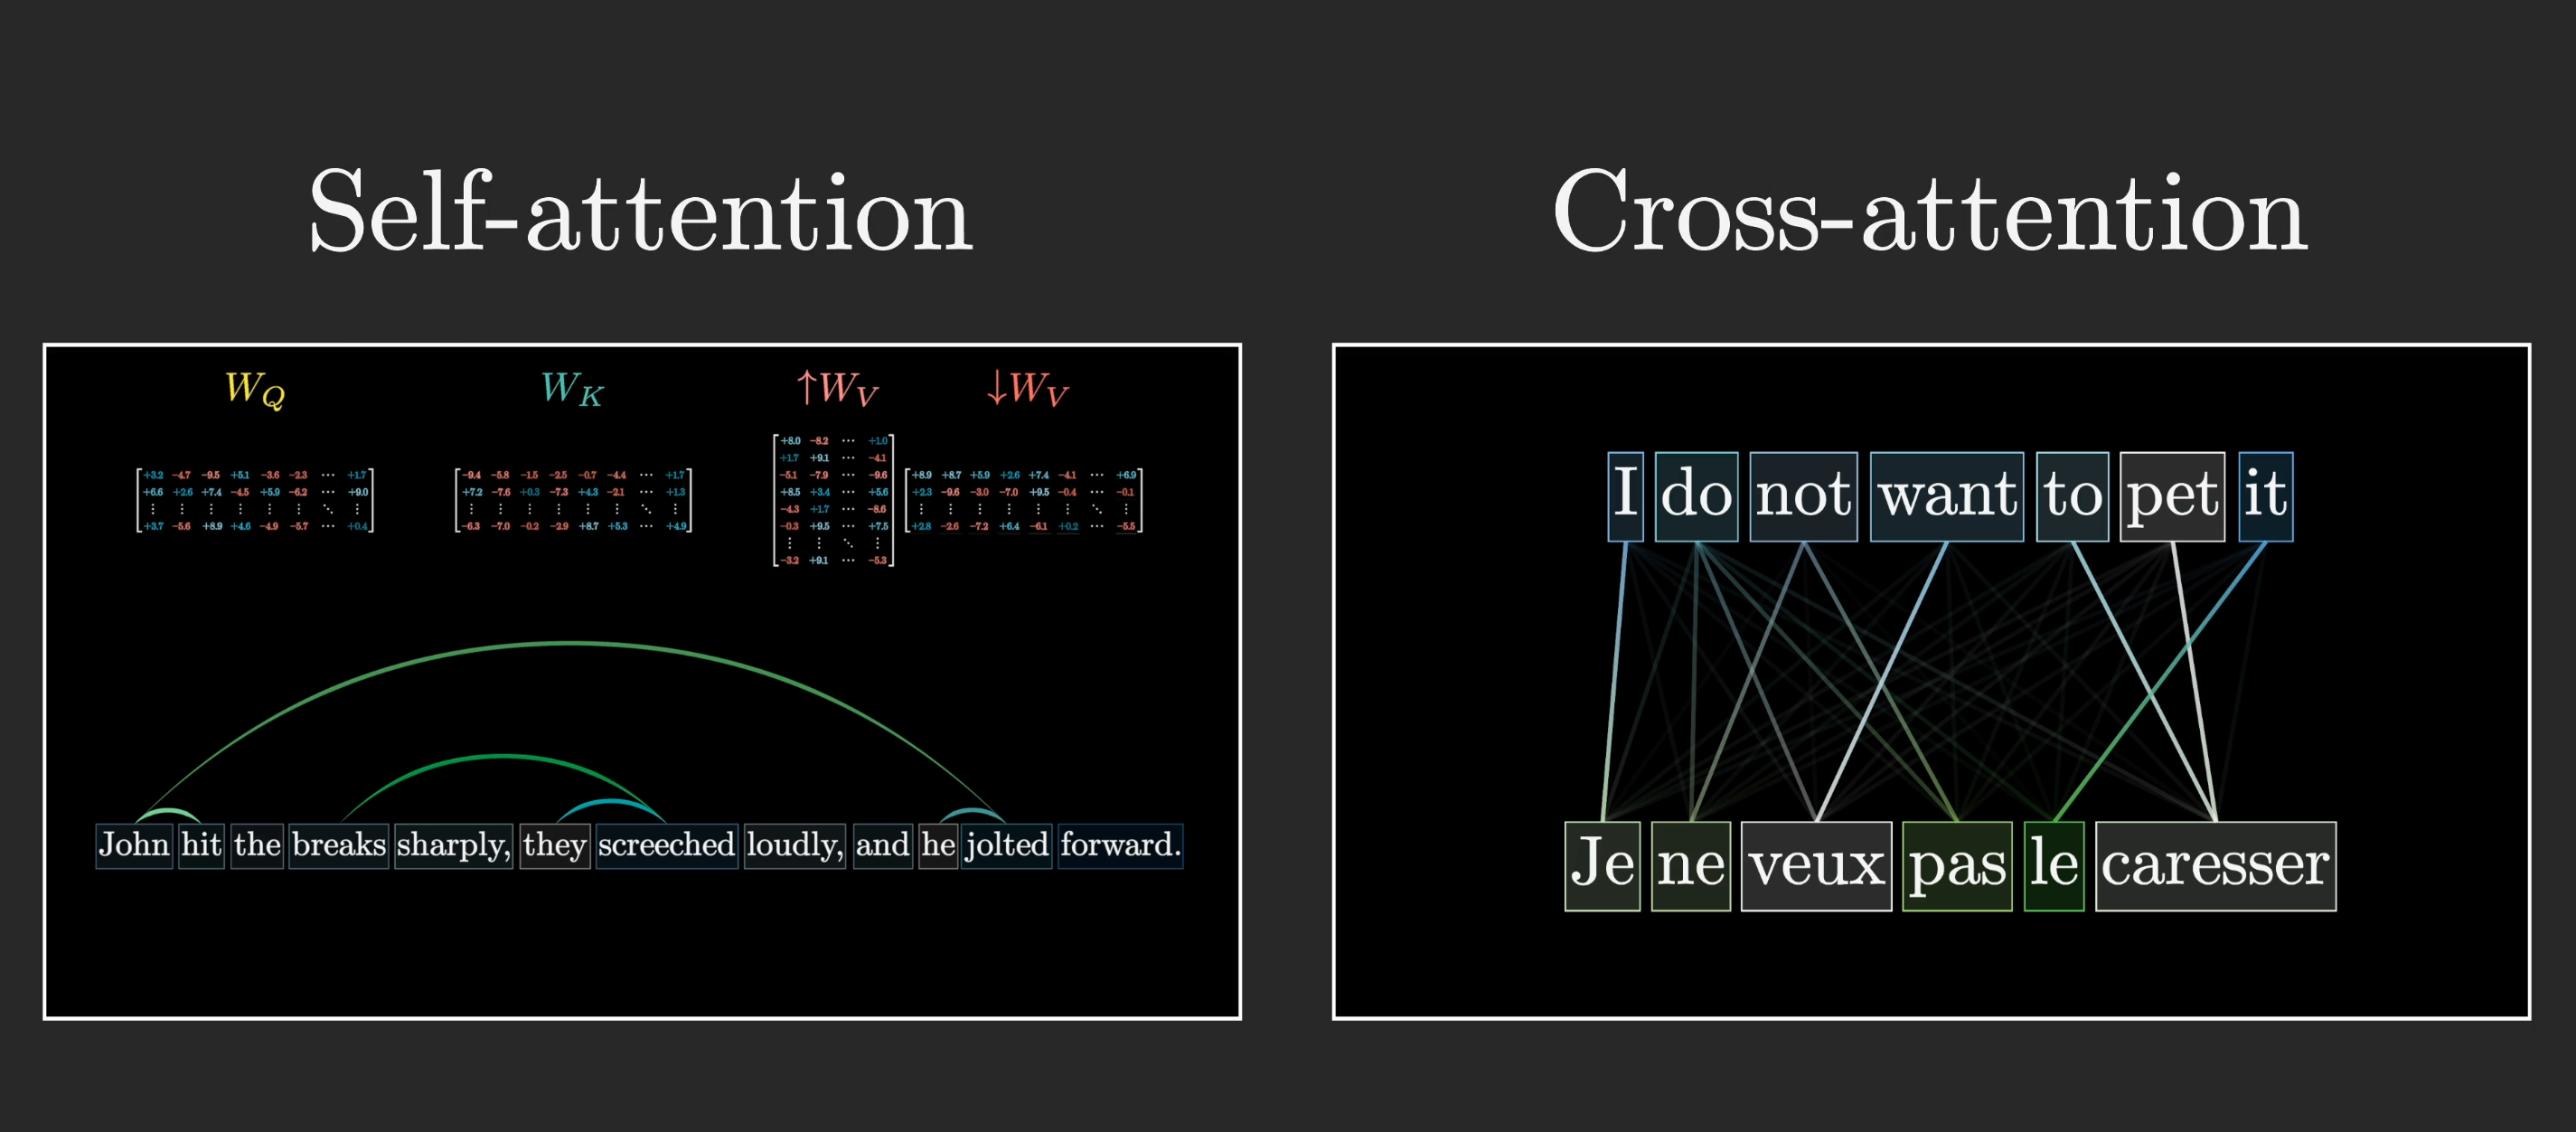
\includegraphics[width=0.95\textwidth, keepaspectratio]{selfXcross_attention.png}
    \end{varwidth}}
    \caption{Визуализация self-attention и cross-attention в контексе задачи NLP \cite{3blue1brown_attention}.}
    \label{fig:selfXcross_attention}
\end{figure}

\paragraph{Multi-Head Внимание}

В механзиме self-attention, описанном выше, всего одна матрица, которая 
описывает сходство между позициями в последовательности. Однако это 
может превратиться в bottleneck архитектуры - было бы полезно, 
чтобы пары точек были похожи в одних измерениях и отличались в других. 

Оказалось выгодным параллельно рассчитывать сразу $H$ наборов self-attention 
($H$ зовутся головами, от англ. Heads) и затем проецировать результаты 
в единственную матрицу, используемую в дальнейших вычислениях. Такого рода 
обобщение называется \textbf{multi-head self-attention} \cite{turner_transformers_intro}
(рис. \ref{fig:multi-head}). \newpage

\begin{figure}[h!]
    \centering
    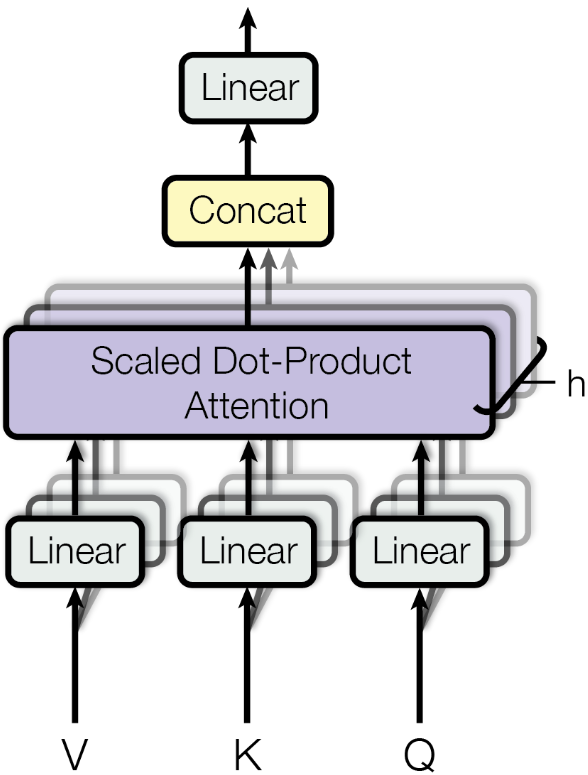
\includegraphics[width=0.35\textwidth, keepaspectratio]{multi-head.png}
    \caption{Multi-Head Attention \cite{vaswani2017attention}.}
    \label{fig:multi-head}
\end{figure}

Multi-head attention позволяет модели совместно воспринимать информацию из 
разных подпространств представлений в разных позициях. При использовании одной 
головы внимания усреднение препятствует этому.
\begin{align*}
    \text{MultiHead($Q$, $K$, $V$)} &= \text{Concat}(\text{head}_1, ..., \text{head}_h)\bm{W}^O, \\
    \text{где } \text{head}_i &= \text{Attention}(\bm{Q}\bm{W}_i^Q, \bm{K}\bm{W}_i^K, \bm{V}\bm{W}_i^V),
\end{align*}
где проекции - матрицы параметров 
$\bm{W}_i^Q \in \mathbb{R}^{d_\text{\tiny model} \times d_k}$, 
$\bm{W}_i^K \in \mathbb{R}^{d_\text{\tiny model} \times d_k}$, 
$\bm{W}_i^V \in \mathbb{R}^{d_\text{\tiny model} \times d_v}$, 
$\bm{W}^O \in \mathbb{R}^{h d_v \times d_\text{\tiny model}}$.

\paragraph{Авторегрессионное маскирование}

Правая часть трансформера (рис. \ref{fig:the_transformer}), представляющая из себя 
декодер также является моделью авторегрессии, тк от нее требуется предсказать 
следущее (в данном случае слово) $w_n$ при заданных предыдщих словах $w_{1:n-1}$, 
т.е. вернуть $p(w_n = w|w_{1:n-1})$. Для успешного выполнения данной операции, нам 
потребуется немного модифицировать наш механизм self-attention. Ранее мы рассматривали 
self-attention как нечто, что собирает контекст для слова как из предыдщих слов в 
предложении, так и из последюущих, однако в случае предсказания новых слов у нас нет 
последующих. Таким образом для корректной работы нашего механизма внимания от нас 
требуется выполнить операцию, известную как \textbf{маскирование (masking)}. 
Грубо говоря, мы зануляем веса в матрице, соответствующие словам, стоящим после рассматриваемого 
(формально говоря мы присваиваем не 0, а $-\infty$, чтобы после применения операции 
$\text{softmax}$ получить валидное распределение).

\subsubsection{Позиционное кодирование}

Поскольку наша модель не содержит ни рекуррентности, ни свертки, для того чтобы 
модель могла пользоваться информацией о порядке последовательности, мы должны 
добавить информацию об относительном или абсолютном положении элементов 
в последовательности. Данного эффекта можно добиться с помощью \textbf{позиционного 
кодирования (positional encoding)}. Существует множество различных видов 
позиционного кодирования, один из них заключается в том, чтобы напрямую включить 
информацию о положении элемента в последовательности в его векторное представление. 
Информация о положении элемента может быть как фиксированной, например 
добавление вектора синусоид различных частот и фаз, чтобы закодировать положение 
слова в предложении (подобный подход как раз и применяется в работе "Attention Is All You Need" 
\cite{vaswani2017attention}), или она может быть свободным обучаемым параметром, 
как это обычно делается в трансформерах для изображений. Также существуют подходы для 
включения информации об относительном расстояним между парами элементов, модифицируя 
механизм self-attention, что наблюдается в эквивариантных трансформерах \cite{turner_transformers_intro}.

\subsubsection{Feed-Forward \& Layer Norm \& Residual connections}

\textbf{Feed Forward Layers. \quad}
Помимо всего рассмотренного, модель трансформера, представленная 
Vaswani et al. \cite{vaswani2017attention}, также включает в себя, так 
называемые, \textbf{слои прямого распространения (Feed Forward Layers)}, которые 
представляют из себя просто многослойные перцептроны (см. главу {\color{red} todo}), 
состоящие из двух линейных преобразований с функцией активации ReLU между ними:
\begin{equation*}
    \text{FFN}(x) = \text{max}(0, \bm{x}\bm{W}_1 + \bm{b}_1)\bm{W_2} + \bm{b_2}
\end{equation*}

\textbf{Layer Norm. \quad}
Плюс, для стабилизации обучения применяется нормировка. Опять же, существует 
множество различных выборов для расчета нормировки, но стандартным подходом считается 
\textbf{LayerNorm}, который нормализует каждый токен по-отдельности, вычитая среднее и 
деля на среднеквадратическое отклонение (что также известно как стандартизация),
\begin{equation*}
    \bar{\bm{x}}_{d,n} = \cfrac{1}{\sqrt{\mathbb{V}[\bm{x}_n]}} 
    (\bm{x}_{d,n} - \text{mean}(\bm{x}_n)) 
    \gamma_d + \beta_d = \text{LayerNorm}(\bm{X})_{d, n},
\end{equation*}
где $\text{mean}(\bm{x}_n) = \frac{1}{D} \sum_{d=1}^D \bm{x}_{d,n}$ и 
$\mathbb{V}(\bm{x}_n) = \frac{1}{D} \sum_{d=1}^D (x_{d,n} - \text{mean}(\bm{x}_n))^2$. 
Параметры $\gamma_d$ и $\beta_d$ - обучаемые параметры масштаба и сдвига.

\begin{figure}[h!]
    \centering
    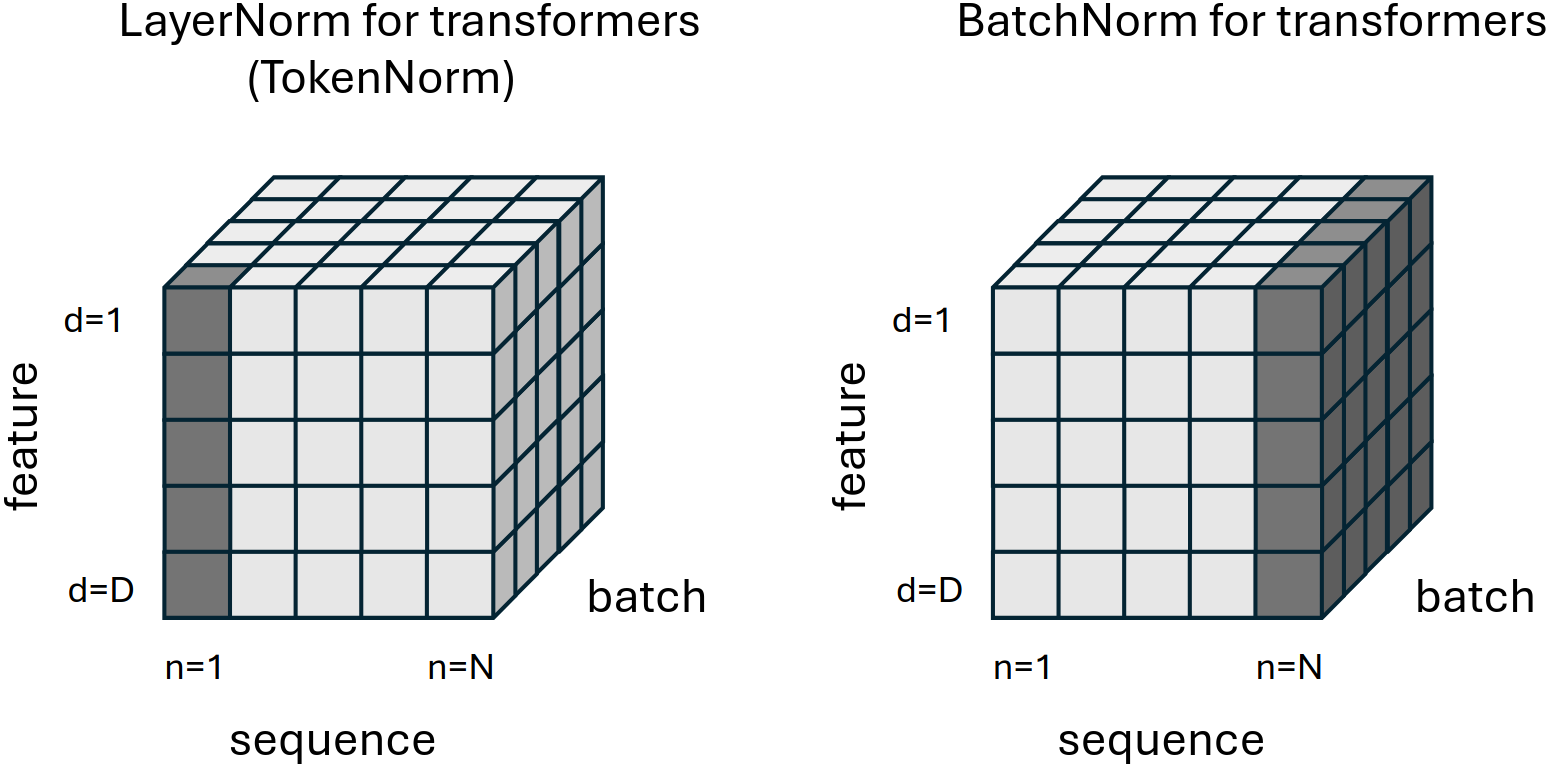
\includegraphics[width=0.8\textwidth, keepaspectratio]{LayerNorm.png}
    \caption{Трансформеры производят layer normalisation (слева), которая 
    нормализует среднее и среднеквадратическое отклонение каждого 
    индивидуального токена в каждой последовательности в бэтче. В 
    свою очередь, batch normalisation (справа), которая нормализует по 
    размерности признака \textit{и} бэтча вместе, на практике показывает себя 
    куда менее стабильной. Разумеется существуют и другие разновидности нормализации. 
    (На данном рисунке автор, во избежание путаницы называет 
    LayerNorm, в применении к трансформерам, TokenNorm, т.к. LayerNorm, 
    в применении к CNN действует иначе) \cite{turner_transformers_intro}.}
    \label{fig:LayerNorm}
\end{figure}

\textbf{Residual connections. \quad}
В машинном обучении широко используют, так называемые, \textbf{остаточные соединения 
(residual connections)}, т.к. они упрощают инициализацию имеют разумный индуктивный 
уклон в сторону простых функций и стабилизируют обучение. Вместо того чтобы напрямую 
указывать функцию $x^{(m)} = f_\theta (x^{(m-1)})$, идея заключается в том, чтобы 
параметризовать ее как тождественное преобразование и остаточный член:
\begin{equation*}
    x^{(m)} = x^{(m-1)} + \text{res}_\theta (x^{(m-1)}).
\end{equation*}

Равнозначно это можно рассматривать как моделирование разностей между 
представлениями $x^{(m)} - x^{(m-1)} = \text{res}_\theta (x^{(m-1)})$ 
и оно будет хорошо работать когда моделируемая функция близка к тождественной 
\cite{turner_transformers_intro}. (Схематично, residual connections представлены 
на рис. \ref{fig:the_transformer} в виде, огибающих блоки, стрелочек, 
ведущих изначальные (до преобразования) величины в блок сложения и нормировки 
(с преобразованными этими же величинами)).

\subsection{Преимущества при моделировании временных рядов}

У трансформеров есть ряд преимуществ при моделировании временных рядов.
\begin{itemize}
    \item \textbf{Распараллеливание.} Благодаря своей природе, трансформеры очень хорошо 
    поддаются распараллеливованию (в отличии от рекуррентных нейронных сетей), из-за 
    чего мы можем обрабатывать гораздо бОльшие объемы данных за то же время.
    \item \textbf{Долгосрочные зависимости.} Одна из ключевых проблем классических 
    рекуррентных нейронных сетей заключается в запоминании долгосроных последовательностей 
    из-за проблемы затухающего градиента. Хорошей попыткой решения данной проблемы 
    послужили LSTM, которые сильно продвинули RNN вперед, однако и у тех, при обработке 
    достаточно длинных последовательностей, возникают проблемы с долгосрочными зависииостями. 
    Механизм внимания полность решает данную проблемы, т.к. в силу отсутствия рекуррентных 
    связей допускает, вообще говоря, бесконечно долгие зависимости.
    \item \textbf{Гибкость.} Трансформеры естественным образом обобщаются на многомерные 
    временные ряды, а также данные с нерегулярной частотой измерений или пропущенными значениями, 
    что делает их универсальным инструментом для анализа временных данных.
\end{itemize}

\subsection{\color{red}Modifications}

% После своего успеха ...

\subsubsection{\color{red}BERT}

% Одной из ключевых проблем в глубоком обучении 
% (продолжим речь в контекст NLP) является нехватка тренировочных данных. 
% Модели современного глубого обучения извлекают огромную выгоду из 
% сильно бОльших объемов данных, улучшаясь при обучении на миллионах, или 
% миллиардах размечанных тренировчных примерах. Для разрешения данной проблемы, 
% исследователи разработали набор техник

\subsubsection{\color{red}GPT}
\subsubsection{\color{red}TFT}
\subsubsection{\color{red}Informer}
% ... 

\subsection{\color{red}State-of-the-art transformers for time series forecasting}

% % % % % % % % % % % % % % % % % % % % % % % %

% state-of-the-art transformers      

% Temporal Fusion Transformer

% Informer
